\chapter{Nuclear physics 3}
\label{nuclear-physics-3}
\section{Nuclear fission}
We have seen a specific case of nuclear fission: the $\alpha$ decay. This process ($\alpha$) is spontaneous and happens by the tunneling effect through the potential barrier (short range) of the nuclear interaction. 
Consider the following fission reaction:
\begin{equation*}
    _{\tiny{Z}}^{\tiny{A}}\mbox{X} \rightarrow _{\tiny{Z}_1}^{\tiny{A}_1}\mbox{X}_1 + _{\tiny{Z}_2}^{\tiny{A}_2}\mbox{X}_2,
\end{equation*}
where $A = A_1 + A_2$ and $Z = Z_1 + Z_2$.
The reaction happens (can happen) if 
\begin{equation*}
    Q_{\tiny{\mbox{fission}}} = M(A,Z) - M(A_1,Z_1) - M(A_2,Z_2) > 0,
\end{equation*}
and 
\begin{equation*}
    Q_{\tiny{\mbox{fission}}} = E_{L}(A,Z) - E_{L}(A_1,Z_1) - E_{L}(A_2,Z_2).
\end{equation*}
The available energy in the nuclear fission processes is typically 0.9 MeV / nucleon. 
Therefore 1 Kg of nucleons equals $6\cdot 10 ^{26}$ nucleons. The energy density will be 
\begin{equation*}
    0.9 \cdot 6 \cdot 10^{26} \mbox{MeV / Kg} = 8.6 \cdot 10^7 \mbox{MJ / Kg}.
\end{equation*}
For comparison, a chemical combustible reaches 20-50 MJ / Kg.


As for the $\alpha$ decay, the fission happens when the atomic number is large and the electrostatic repulsion between the nuclei become strong. Following the liquid drop model, we can imagine the fission process as the splitting process of a liquid drop, as represented in Figure \ref{fig:nuclear-physics3-fig1}.
\begin{figure}
    \centering
    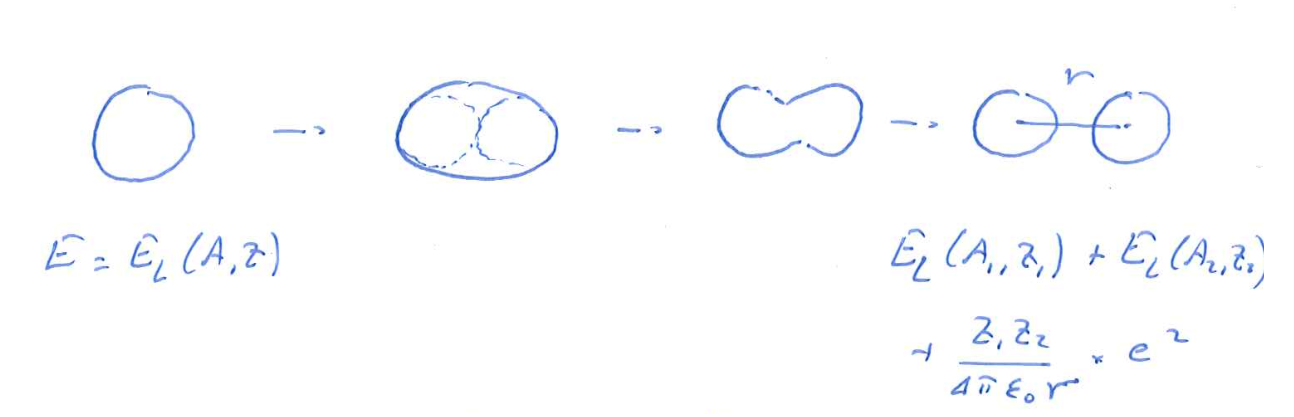
\includegraphics[width=0.8\textwidth]{Figures/nuclear-physics3-fig1}
    \caption{Liquid drop separation as a model of nuclear fission}
    \label{fig:nuclear-physics3-fig1}
\end{figure}

The system can be visualised through a potential, where the nucleus exists if it exists a meta-stable state, as represented in Figure \ref{fig:nuclear-physics3-fig2}.
\begin{figure}
    \centering
    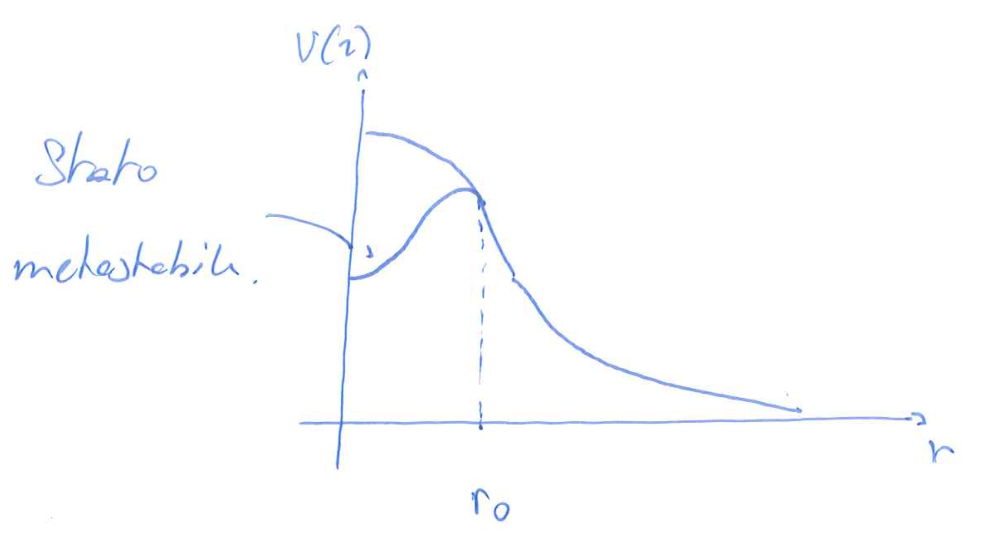
\includegraphics[width=0.8\textwidth]{Figures/nuclear-physics3-fig2}
    \caption{Potential energy as a function of the radius from the nucleus centre.}
    \label{fig:nuclear-physics3-fig2}
\end{figure}
For nuclei with large value of A, the spontaneous fission typically happens promptly, and a meta-stable state does not exist. For some nuclei like the $^{238}\mbox{U}$ the spontaneous fission through tunnelling effect can happen, but has an half-life $T_{1/2} \sim 10^{15} \mbox{yr}$.

The spontaneous fission becomes the main process that, probably, forbids the formations of extremely heavy nuclei. 

\section{Stability and fission}
Let's consider an ellipsoid (instead of a sphere).
\begin{figure}
    \centering
    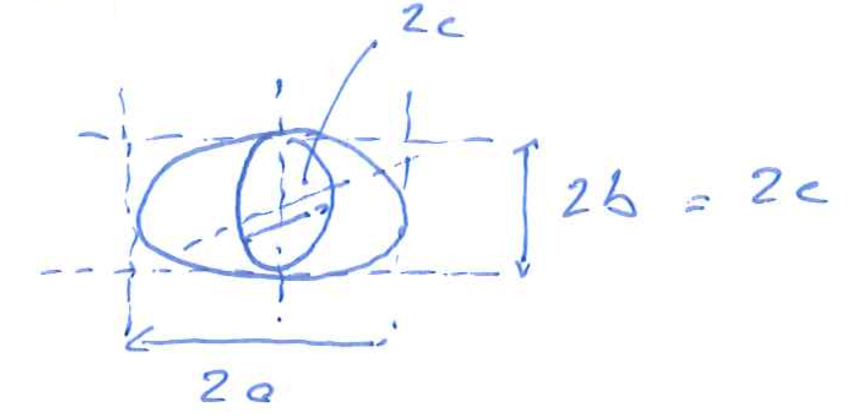
\includegraphics[scale=0.5]{Figures/nuclear-physics3-fig3.pdf}
    \caption{Illustration of the ellipsoid model for Nucleus}
    \label{fig:nuclear-physics3-fig3}
\end{figure}
We assume that the nucleus is incompressible, therefore the volume is constant
\begin{equation*}
    V = \frac{4}{3}\pi ab^2 = \frac{4}{3}\pi r^3.
\end{equation*}
The deformations can be parametrized as 
\begin{equation*}
    a = r(1+\epsilon) \;\;\;\;,\;\;\;\; b = \frac{r}{\sqrt{1+\epsilon}}.
\end{equation*}
The volume term in the Bethe Weizsaecker equation does not change, while the surface term $a_2A^{2/3}$ becomes $a_2A^{2/3}(1+\frac{2}{5}\epsilon^2)$.
The surface of the ellipsoid is given by
\begin{equation*}
    S = 4\pi r^2 \left(1+\frac{2}{5}\epsilon^2\right).
\end{equation*}
Also the electrostatic energy term is modified in a non trivial way
\begin{equation*}
    U = \frac{1}{2}\int \int \frac{1}{4\pi\epsilon_0} \frac{\rho(r1)\rho(r2)dr_1dr_2}{r_{12}}.
\end{equation*}
The non trivial integral for the ellipsoid yield to:
\begin{equation*}
    U = U_{\tiny\mbox{sphere}} \times \left(1-\frac{\epsilon^2}{5}\right),
\end{equation*}
therefore
\begin{equation*}
    a_3 \frac{Z^2}{A^{1/3}} \rightarrow a_3 \frac{Z^2}{A^{1/3}}\left(1-\frac{\epsilon^2}{5}\right),
\end{equation*}
and in the end
\begin{equation*}
    U = \frac{3}{5}\frac{1}{4\pi\epsilon_0}\frac{Q^2}{R}\left(1-\frac{\epsilon^2}{5}\right).
\end{equation*}


We find that:
\begin{itemize}
    \item the surface energy term increases;
    \item the electrostatic term decreases.
\end{itemize}
The changes to the Bethe-Weizsaecker equation are:
\begin{equation*}
    a_2A^{2/3}\left(1+\frac{2}{5}\epsilon^2\right)+a_3\frac{Z^2}{A^{1/3}}\left(1-\frac{\epsilon^2}{5}\right) = a_2A^{2/3} + a_3\frac{Z^2}{A^{1/3}} + \left(\frac{2}{5}A^{2/3}a_2 - \frac{a_3}{5}\frac{Z^2}{A^{1/3}}\right) \epsilon^2,
\end{equation*}
and therefore the difference in energy $\Delta E$ between the sphere and the ellipsoid will be:
\begin{equation*}
    \Delta E = \frac{2}{5}a_2A^{2/3}\left(1-\frac{a_3}{2a_2}\frac{Z^2}{A}\right) \epsilon^2.
\end{equation*}
The spherical nucleus will be stable if $\Delta E > 0$, and therefore:
\begin{equation*}
    \Delta E \sim \frac{2}{3}a_2A^{2/3}\left(1-\frac{1}{50}\frac{Z^2}{A^{1/3}}\right)\epsilon^2,
\end{equation*}
using the coefficients $a_2$ and $a_3$ discussed before we find
\begin{equation*}
    \frac{Z^2}{A} < 50,
\end{equation*}
which holds also for very heavy nuclei. This means that the spontaneous fission is not obvious.

\section{Induced fission}
Through collision with other particles, and in particular with neutrons, the potential barrier of the fission process can be reduced. For the isotope $^{235}\mbox{U}$ the threshold kinematic energy of neutron to obtain the fission is very low (similar happens for the Plutonium)
\begin{equation*}
    E < 0.1 ~\mbox{eV}.
\end{equation*}
With the capture of a neutron, the $^{235}\mbox{U}$ becomes $^{236}\mbox{U}$ which is a even-even nucleus, which has a negative paring term ($a_5$ in the Bethe-Weizsaecker formula). For the $^{235}\mbox{U}$ this is null, being A odd. The fission threshold for the $^{238}\mbox{U}$ with neutron capture is much more higher, $> 2 ~\mbox{MeV}$.

$^{235}\mbox{U}$ is in the 0.7\% of the natural uranium and goes under fission with low energy neutrons, called \emph{thermal}. A neutron is \emph{thermal} when the kinetic energy of the neutron is comparable to the one of the surrounding atoms (the neutrons are slowed down to the thermal equilibrium). 
\begin{equation*}
    kT = 25 ~\mbox{meV}\,\,\,\,\mbox{at 300 K}.
\end{equation*}


The $^{235}\mbox{U}$ is the only fissile material with fission induced by thermal neutrons which is enough abundant in nature. Fissile materials can be produced from fertile materials, as the $^{239}\mbox{Pu}$, $^{233}\mbox{U}$ from the $^{238}\mbox{U}$ and $^{232}\mbox{Th}$. There are auto-fertilizing reactors which burn $^{239}\mbox{Pu}$ and produce $^{239}\mbox{Pu}$ from $^{238}\mbox{U}$.

\begin{figure}[h!]
    \centering
    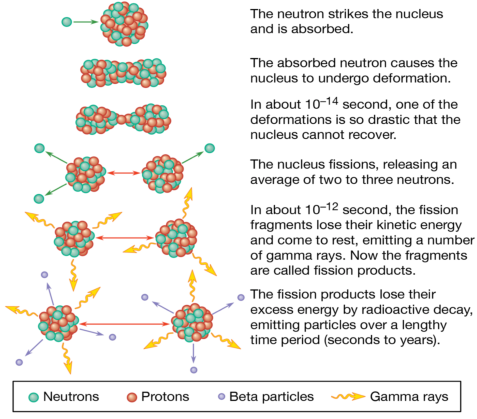
\includegraphics[width=1\textwidth]{Figures/nuclear-physics3-fig4.pdf}
    \caption{Scheme of the induced fission.}
    \label{fig:nuclear-physics3-fig4}
\end{figure}

\begin{figure}
    \centering
    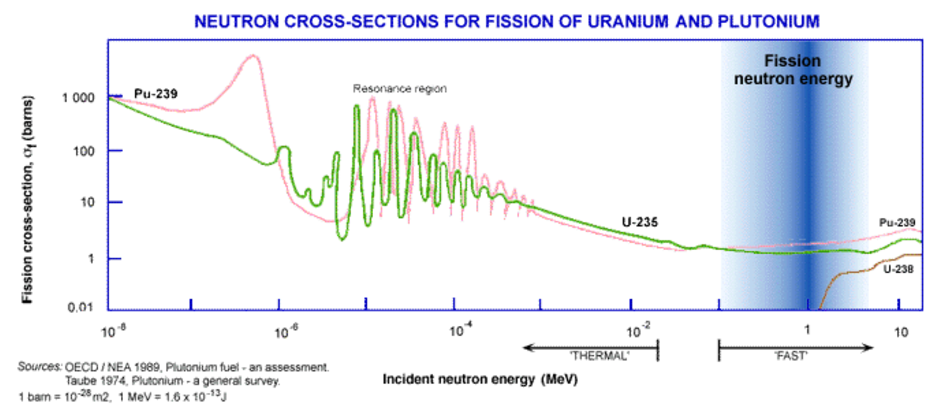
\includegraphics[width=0.8\textwidth]{Figures/nuclear-physics3-fig5.pdf}
    \caption{}
    \label{fig:nuclear-physics3-fig5}
\end{figure}

\section{Chain reactions}
The chain reaction is the base principle of the nuclear reactors.
\begin{equation*}
    \mbox{n} + ^{235}\mbox{U} \rightarrow 
    \mbox{Fission products} + 2.5 ~\mbox{neutron (mean)}
\end{equation*}
For example:
\begin{equation*}
    _{\tiny{0}}^{\tiny{1}}\mbox{n} ~+~ _{\tiny{92}}^{\tiny{235}}\mbox{U}~ \rightarrow~ _{\tiny{92}}^{\tiny{236}}\mbox{U}~ \rightarrow~
    _{\tiny{56}}^{\tiny{141}}\mbox{Ba} ~+~ _{\tiny{36}}^{\tiny{92}}\mbox{Kr} ~+~ 3~_{\tiny{0}}^{\tiny{1}}\mbox{n}.
\end{equation*}
When the nucleus breaks, it generates:
\begin{itemize}
    \item neutrons;
    \item nuclei (and other $\beta$ and $\gamma$ decays) with kinetic energy which generates heat in the material; 
    \item emitted neutrons emitted by produced nuclei, called \emph{delayed neutrons}.
\end{itemize}
Produced neutrons can also be captured by other nuclei and produce a chain reaction, as represented in Figure \ref{fig:nuclear-physics3-fig6}.

\begin{figure}
    \centering
    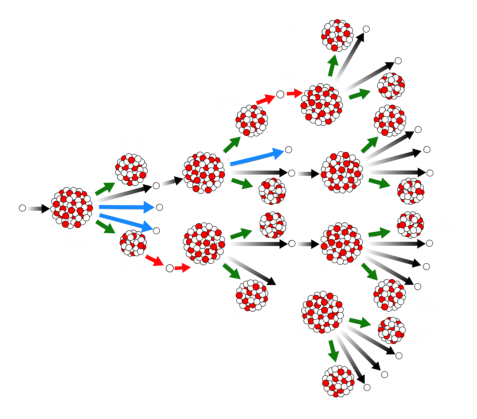
\includegraphics[scale=1.2]{Figures/nuclear-physics3-fig6.pdf}
    \caption{Chain reaction. The blue arrows indicate the late emission of neutrons. The red arrows indicate the capture of neutrons by other nuclei.}
    \label{fig:nuclear-physics3-fig6}
\end{figure}

A fundamental aspect of the chain reaction is its control:
\begin{itemize}
    \item an insufficient production of neutrons stops the chain;
    \item an over-production of neutrons leads to an exponential process which lead to the \emph{explosion} of the system.
\end{itemize}
The reaction chain can be modelled in the following way:
\begin{itemize}
    \item N(t): number of neutrons;
    \item $\tau$: mean time for a neutron to produce a primary fission;
    \item $\nu$: mean number of neutrons produced in a fission process;
    \item q: probability for a neutron to produce a fission (taking into account the absorbed neutrons which does not produce any fissions).
\end{itemize}
For each passage from a geneartion \emph{i} to the next one \emph{i+1} we have a variation dN which can be written as:
\begin{equation}
    \frac{\mbox{dN}}{\mbox{N}} = \lambda (-1 + \nu q)~dt
    \label{eq:nuclear-physics3-eq1}
\end{equation}
where the -1 is due to the primary fission while the term $\nu q$ accounts for the effective neutrons. Integrating and posing $\lambda=\frac{1}{\tau}$ we have
\begin{equation*}
    \mbox{N}(t) = \mbox{N}(0)~ e^{(\nu q -1)\frac{t}{\tau}},
\end{equation*}
where:
\begin{itemize}
    \item for $\nu q < 1$ the regime is called \emph{sub-critical}, and the chain reaction does not develop. The number of neutrons decrease with time;
    \item for $\nu q = 1$ the regime is called \emph{critical}, and the number of neutrons (and secondary fission processes) is stable;
    \item for $\nu q > 1$ the regime is called \emph{super-critical}, the number of reactions increases exponentially.
\end{itemize}

\section{Cross section and critical mass}
The neutrons generated in the fission process can undergo several processes:
\begin{itemize}
    \item they can be captured by nuclei, emitting $\gamma$ radiation (without producing fission) - $\sigma_{n,\gamma}$;
    \item can do elastic scattering or loose energy through inelastic scattering processes;
    \item produce a new fission process - $sigma_{\tiny\mbox{fission}}$.
\end{itemize}
Typically neutrons loose energy through collisions. The factor $q$ in Equation \ref{eq:nuclear-physics3-eq1} can be written as 
\begin{equation}
    q = \frac{\bar{\sigma}_{\tiny\mbox{fission}}}{\bar{\sigma}_{\tiny\mbox{fission}} + \bar{\sigma}_{n,\gamma}}.
\end{equation}
For $^{238}\mbox{U}$ and $T_{\tiny\mbox{neutron}} = 2~\mbox{MeV}$:
\begin{itemize}
    \item $\sigma_{\tiny{\mbox{tot}}} = 7.3~\mbox{b}$;
    \item $\sigma_{\tiny{\mbox{fission}}} = 0.53~\mbox{b}$;
    \item $\sigma_{n,\gamma} = 0.048~\mbox{b}$.
\end{itemize}
Therefore most of the collisions are scattering with loss of energy in which the neutron is not absorbed.
For the $^{238}\mbox{U}$ with $T_{n} = 2~\mbox{MeV}$ the picture is similar:
\begin{itemize}
    \item $\sigma_{\tiny{\mbox{tot}}} = 7.15~\mbox{b}$;
    \item $\sigma_{\tiny{\mbox{fission}}} = 1.89~\mbox{b}$;
    \item $\sigma_{n,\gamma} = 0.059~\mbox{b}$.
\end{itemize}
\begin{figure}
    \centering
    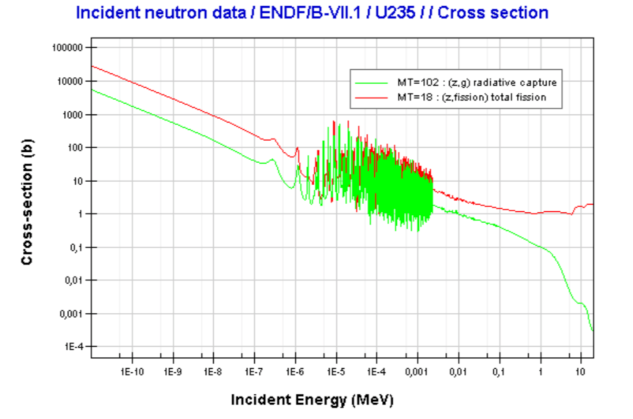
\includegraphics{Figures/nuclear-physics3-fig7.pdf}
    \caption{Cross section as a function of incident energy for $^{235}\mbox{U}$.}
    \label{fig:nuclear-physics-fig7}
\end{figure}
The situation totally changes for thermal neutrons with a kinematic energy of 25 meV ($25 \cdot 10^{-3}~\mbox{eV}$):
\begin{table}[]
    \centering
    \begin{tabular}{|c|c|c|c|}
         \hline
         & $\sigma_{\tiny{\mbox{tot}}}$ & $\sigma_{\tiny{\mbox{fission}}}$ & $\sigma_{n,\gamma}$ \\
         \hline
        $^{235}\mbox{U}$ & 703 b & 589 b & 95 b \\
        \hline
        $^{238}\mbox{U}$ & 12 b & $2\cdot10^{-5}$ b & 2.7 b \\
        \hline
    \end{tabular}
    \caption{Resume table of cross section for two isotopies of U(for neutrons of 2 Mev)}
    \label{tab:nuclear-physics3-tab1}
\end{table}
For neutrons of 2 MeV, the cross section is low for both $^{235}\mbox{U}$ and $^{238}\mbox{U}$. While for $^{235}\mbox{U}$ and $T_{n} = 25~\mbox{meV}$ the cross section is two orders of magnitude higher.
For energies lower than 2 MeV (fission threshold of the $^{238}\mbox{U}$) the condition q $<< 1$ is easily verified since the neutrons are mainly subject to scattering without any absorption process, and therefore they loose energy.


$T_{n} = 2~\mbox{MeV}$ is exactly the mean kinetic energy of the neutrons emitted through the fission process. 
\begin{figure}
    \centering
    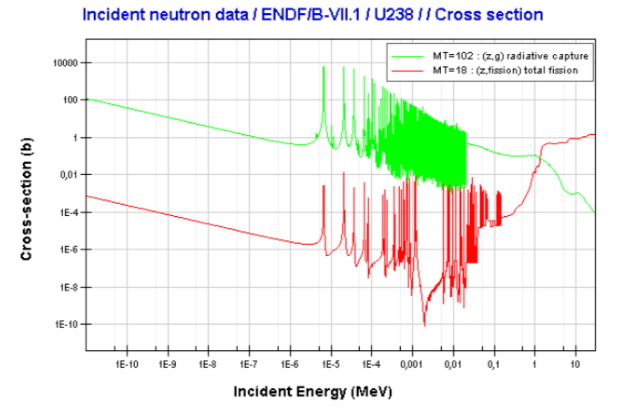
\includegraphics{Figures/nuclear-physics3-fig8.pdf}
    \caption{Cross section as a function of incident energy for $^{238}\mbox{U}$.}
    \label{fig:nuclear-physics-fig8}
\end{figure}

\section{Principles of nuclear reactors}
A nuclear reactor is typically composed by the following elements:
\begin{itemize}
    \item \emph{combustible}: contains $^{235}\mbox{U}$ and $^{238}\mbox{U}$;
    \item \emph{absorber}: material to absorb neutrons (Boron, Argon, Cadmium);
    \item \emph{moderator}: material to thermalise neutrons (H$_2$O, graphite, Beryllium);
    \item \emph{heat exchanger}: mean to exchange heat and transfer it, in order to generate electric current.
\end{itemize}
Through several reactions and absorption it is possible to maintain the reactor in the \emph{critic} state, meaning that the reaction is controlled and the system in stable. The critic regime is the normal functioning state of a reactor. 

The critical regime is also related to the mean path of the neutrons before they are captured or initiate another fission process. Therefore it exists a minimum distance needed for the reaction in order to self-sustain, and therefore it exists a critical volume, or critical \emph{mass}, which can be evaluated. This critical mass is controlled through the use of the absorbers, which are used to control the chain reaction.

\begin{figure}
    \centering
    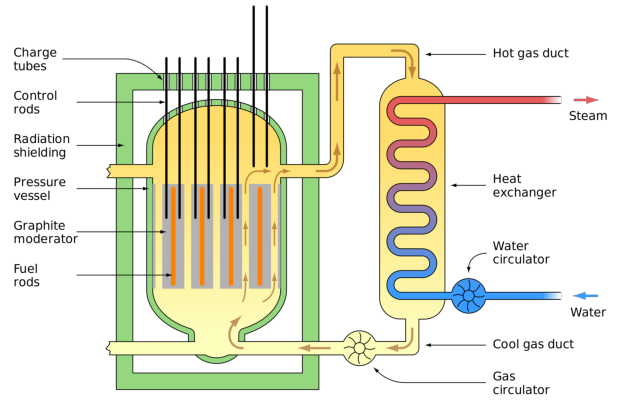
\includegraphics{Figures/nuclear-physics3-fig9.pdf}
    \caption{Scheme of a nuclear reactor with: gas (CO$_2$) heat exchanger, natural Uranium as combustible, Boron as absorber, graphite as moderator element.}
    \label{fig:my_label}
\end{figure}

\section{Nuclear fusion}
The nuclear fusion is the process active in our Sun which produces energy. Taking the easiest fusion process:
\begin{equation*}
    p~+~p \rightarrow ^{2}\mbox{H}~+~e^{+} + \nu_e
\end{equation*}
it is clear that there is a Coulombian potential barrier to be overtaken before the two protons can form a bounded state, with a typical distance of $~1~\mbox{fm}$ (keep in mind that the weak nuclear force acts on distances of the order $~10^{-18}~\mbox{m}$).

In order to overtake the Coulombian potential barrier it is needed an energy of about
\begin{equation*}
    V_{pp} = \alpha\frac{\hslash c}{2r}Z_{x}Z_{y} \sim 0.7 ~\mbox{MeV}. 
\end{equation*}
Being the temperature in the centre of the sun of about $T \sim 15 \times 10^6~\mbox{K}$, the mean energy of the protons will be about
\begin{equation*}
    kT \sim 1.3\mbox{keV},
\end{equation*}
which is about 600 times less than the needed energy to overtake the potential barrier. In order for this reaction to happen it is necessary that the process happens through the tunnelling effect (similar to the fission process or the emission of $\alpha$ particles). This comes with a similar factor to the Gamow one for the $\alpha$ particle emission.

\subsection{Fusion processes in the Sun}
Here the fusion processes which are happening in the Sun will be presented, which are made by two main cycles:
\begin{itemize}
    \item the pp cycle (proton-proton chain) transforms protons in Helium. This cycle is made by several branches which go through heavier elements like Beryllium or Boron, but end in He;
    \item the CNO cycle, which starting from Carbon Helium 4 is produced through the following reactions:
    \begin{equation*}
    \begin{split}
        &^{12}C~+~p ~ \rightarrow ~ ^{13}\mbox{N}~+~\gamma + 1.95~\mbox{MeV}\\
        ^{13}N ~ \rightarrow ~ ^{13}\mbox{C}~+~ e^+ ~+~ \nu_e ~+~ &1.37~\mbox{MeV}\\
        ^{13}C ~+~p \rightarrow ~ ^{14}\mbox{N}~+~\gamma + 7.94~\mbox{MeV}\\
        &^{14}N ~+~p \rightarrow ~ ^{15}\mbox{O}~+~\gamma + 7.39~\mbox{MeV}\\
        &^{15}O ~\rightarrow ~ ^{15}\mbox{N}~+~ e^+ + \nu_e + 1.86~\mbox{MeV}\\
        &^{15}N ~+~ p ~\rightarrow ~ ^{12}\mbox{C}~+~ ^{4}\mbox{He} + 4.96~\mbox{MeV}\\
    \end{split}
    \end{equation*}
    With the provision of 4 protons $^{4}\mbox{He}$ can be produced.
\end{itemize}
\begin{itemize}
        \item These reactions produce energy;
        \item These reactions produce neutrinos!
    \end{itemize}
\begin{figure}
    \centering
    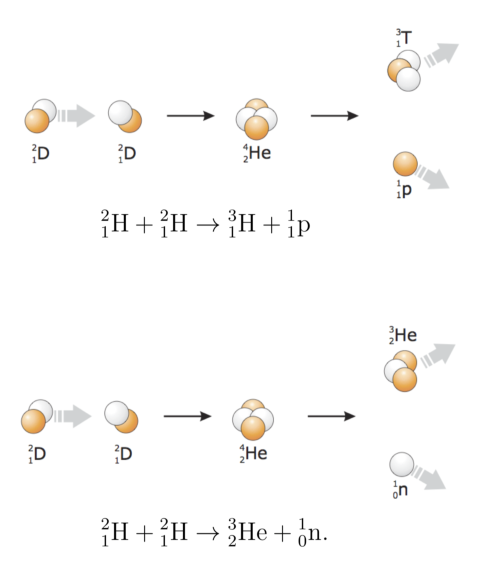
\includegraphics[width=0.8\textwidth]{Figures/nuclear-physics3-fig10.pdf}
    \caption{}
    \label{fig:nuclear-physics3-fig10}
\end{figure}

\begin{figure}
    \centering
    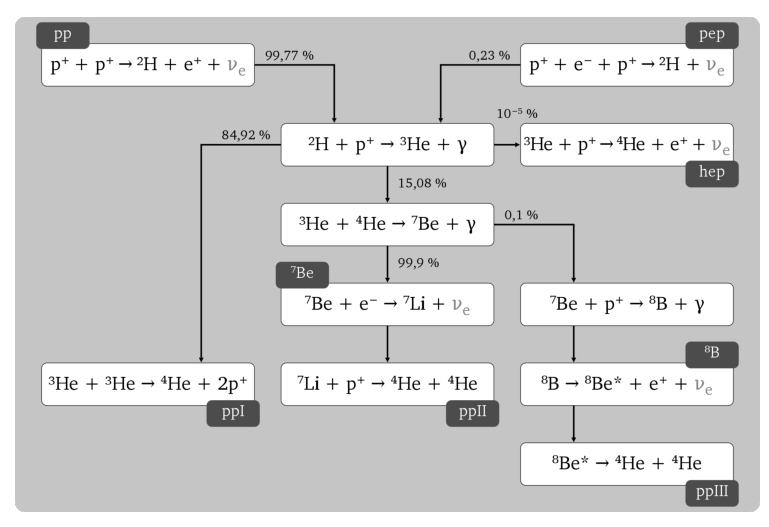
\includegraphics[width=0.8\textwidth]{Figures/nuclear-physics3-fig11.pdf}
    \caption{}
    \label{fig:nuclear-physics3-fig11}
\end{figure}

\begin{figure}
    \centering
    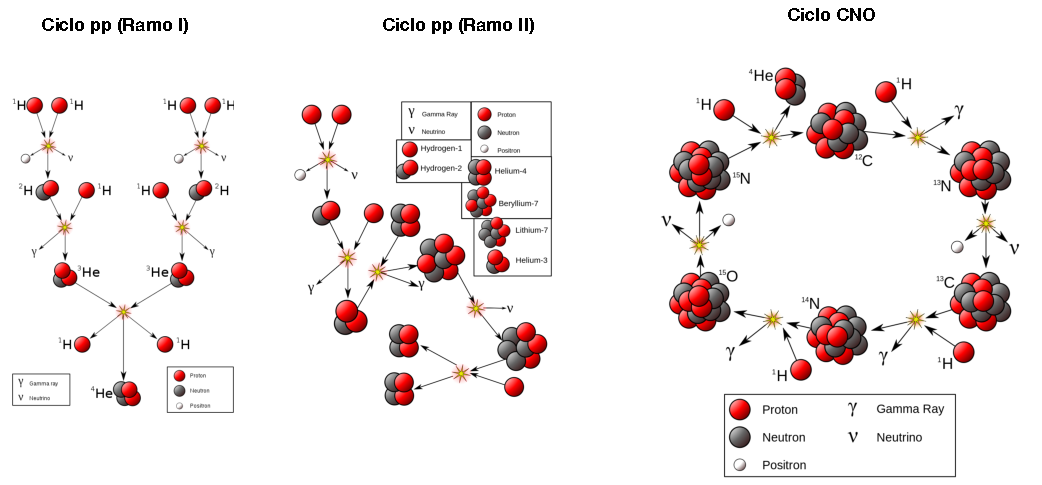
\includegraphics[width=0.8\textwidth]{Figures/nuclear-physics3-fig12.pdf}
    \caption{}
    \label{fig:nuclear-physics3-fig12}
\end{figure}